\documentclass[12pt]{article}

\newcommand\tab[1][1cm]{\hspace*{#1}}

\usepackage{times}
\usepackage{amsmath}
\usepackage{fullpage}
\usepackage{latexsym}
\usepackage{graphicx}
\usepackage{amsfonts}

\graphicspath{ {./images/} }

\newcommand{\NOT}{\neg}
\newcommand{\AND}{\wedge}
\newcommand{\OR}{\vee}
\newcommand{\XOR}{\oplus}
\newcommand{\IMPLIES}{\rightarrow}
\newcommand{\IFF}{\leftrightarrow}
\newcommand{\E}{\exists}
\newcommand{\A}{\forall}

\setlength{\parskip}{.1in}

\renewcommand{\baselinestretch}{1.1}

\begin{document}

\begin{center}

{\bf
CSCE 313\\
Quiz 5\\
Jeffrey Xu\\
11/19/20\\
}

\end{center}

\section{True/False}

{\bf 1.} UDP protocol deals with retransmitting packets in case they are lost in route.

{\bf Solution:}\\

False. UDP just sends out packets and doesn't really retransmit packets. 

{\bf 2.} TCP protocol is more heavy-weight because it maintains state information about the connection.

{\bf Solution:}\\
True. TCP stores the state of the connection and deals with issues that may arise if there are issues with the connection. 

{\bf 3.} Routing protocols are dynamic: they reconfigure under network topology change or outage automatically.

{\bf Solution:}\\

True. Most routing protocols are dynamic and can adjust the settings and states based on the current condition of routers and connections. 

{\bf 4.} Domain Naming System (DNS) can be used for load balancing and faster content delivery.

{\bf Solution:}\\

True. DNS facilitates faster access to domains by providing several IP addresses for a single host or domain name. This allows for traffic to go through multiple servers. 

{\bf 5.} The ping command is used to test whether you can make TCP connections with a remote host.

{\bf Solution:}\\

True. The ping command simply checks if you can connect to a remote host, not if you can make a TCP connection with a remote host. 

{\bf 6.} The accept() function needs to be called the same number of times as the number of client-side connect() calls to accept all of them. 

{\bf Solution:}\\

True. 

{\bf 7.} HTTP protocol uses TCP underneath.

{\bf Solution:}\\

True.

{\bf 8.} Ports [0,1023] are reserved for well-known services (e.g., HTTP, SMTP, DNS, TELNET).

{\bf Solution:}\\

True. 

{\bf 9.} The master socket in a TCP server is used only to accept connections, not to run conversations with clients. 

{\bf Solution:}\\

True. The master socket accepts connections then redirects the client to other sockets to actually perform the conversations. 

{\bf 10.} A socket is a pair of IP-address and port number combination in both client and server side. 

{\bf Solution:}\\

True. 

{\bf 11.} For making a socket on the client side, the port number is chosen by the OS randomly from the available pool.

{\bf Solution:}\\

True. 

{\bf 12.} A socket is like other file descriptors and is added to the Descriptor Table. 

{\bf Solution:}\\

True. Sockets have indices in the file descriptor table in UNIX systems. 

{\bf 13.} UDP is connectionless while TCP is connection oriented. 

{\bf Solution:}\\

True. 

{\bf 14.} The ping command is used to test network reachability.

{\bf Solution:}\\

True. The ping command tests whether a remote host can be connected to. 

{\bf 15.} The bind() function is used to set up a backlog of outstanding connections. 

{\bf Solution:}\\

False. The bind command associates a socket to a given port. 

\section{Short Answers}

{\bf 16. [20 pts]} Consider a disk that has 10 ms seek latency, 0.1ms rotational latency and 250MB/sec read speed. How much time would it take to read:

{\bf a. [10 pts]} One file size 1MB. 

{\bf Solution:}\\

We know that disk access time = seek time + rotation time + transfer time. The total time is $(10ms)+(0.1ms)+(1/250s)$ which gives a total time of $14.1ms$. 

{\bf b. [10 pts]} 100 files each of size 1 byte. Assume they are scattered randomly through the disk. 

{\bf Solution:}\\

Here, we can calculate the total time as $(100*(10ms+0.1ms))+100*(1/250000000s)=1010.0004ms$. 

{\bf 17. [25 pts]} A file system consists of disk blocks that are 32KB and pointers to blocks are each 16 bytes each. Each inode in this file system contains 10 direct pointers, 1 single indirect, 1 double indirect and 2 triple indirect pointers. Now, in this file system:

{\bf a. [10 pts]} What is the maximum possible file size?

{\bf Solution:}\\

We know that each disk block has a size of 32KB. Since each pointer takes 16 btyes, we have that each block can store $2^{11}$ pointers. Therefore, we can compute the total size as follows.

\begin{center}
$32KB[10+2^{11}+2^{22}+2*2^{33}]=549890097472KB$\\
\end{center}

This is approximately 512TB (512.125TB) as the maximum file size. 

{\bf b. [15 pts]} What is the overhead to represent this maximum-size file?

Now we need to determine the amount of space needed to store the overhead for this file size. We would still need 17184065546 pointers and each pointer takes 16 bytes. Therefore, we get a total of 17184065546*16 bytes which is 274945048736 bytes (approximately 256GB or 256.063TB) to store the overhead. 

{\bf 18. [40 pts]} Examine the Tannenbaum’s solution to the Dining-Philosophers problem posted in the following: https://legacy.cs.indiana.edu/classes/p415-sjoh/hw/project/dining-philosophers/index.htm.

{\bf a. [25 pts]} Rewrite the given solution in C++ using the semaphore class from our class lecture, make sure the program compiles and runs. Test the program and verify that it works correctly and show that using screenshots.

{\bf Solution:}\\

A screenshot of the output produced by the code is shown below. 

\begin{center}
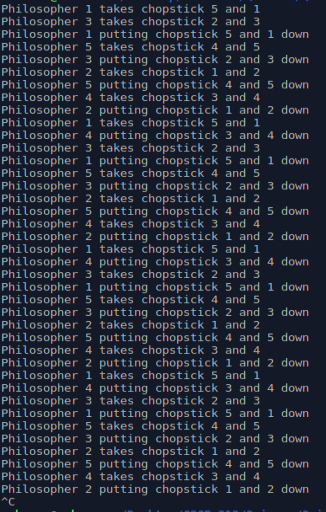
\includegraphics[width=6cm, height=14cm]{q18Output}
\end{center}

The code used to produce this output is attached. The code compiles and runs perfectly. 

{\bf b. [15 pts]} Then, describe how this solution works and why it does not run into deadlocks.

{\bf Solution:}\\

The main idea of the philosopher function is that each philosopher goes through a cycle of taking chopsticks and putting down chopsticks. We have a Semaphore called $m$ that basically protects the state of each philosopher. We also have another vector of Semaphores that protects each philosopher. The code works correctly and doesn't have deadlocks because each time a philosopher tries to take chopsticks, it must check that the chopsticks are available before picking them up (it does this by checking that the philosopher to the left and right of the current philosopher aren't eating). Otherwise it doesn't pick up the chopsticks and waits (using the Semaphore) until the chopsticks are free and then they pick up the chopsticks. Since each Semaphore is used properly, there cannot be any deadlocks in the code. 

\end{document}